
Earth observation satellites play an important role for many scientific and
meteorological applications. Their unique ability to provide frequent
observations of large parts of the globe allows meteorologists to predict the
weather and scientists to study the Earth and its atmosphere. Weather
predictions as well as the monitoring of the  climate are of considerable
societal and economical value; a value that is likely to increase as the 
Earth continues to warm.

Observations from these satellites consist of measurements of electromagnetic
radiation, which is either reflected or emitted from the Earth and its
atmosphere. An example of such measurements is given in
Fig.~\ref{fig:introduction:water_vapor}. Besides demonstrating its delicate
beauty, this image of infrared radiation emitted from a low pressure system over
the Mediterranean sea contains valuable information about the physical state of
the atmosphere. The colors in the image represent the intensity of the measured
radiation from strong to weak using bright to dark colors. At this specific
wavelength, the measured radiation stems from water vapor and clouds in the
atmosphere. This makes dry air less opaque and allows the satellite to sense
radiation from lower down in the atmosphere. Since the temperatures in the lower
atmosphere increase with decreasing height, the radiation in these regions is
more intense. Bright colors thus identify regions of relatively dry air. Moist
air, which is more opaque, emits radiation from higher up in the atmosphere
where temperatures are lower and thus produces the moderate intensities in the
image. The lowest intensities stem from high clouds, which are fully opaque and
thus emit radiation at  high altitudes and low atmospheric temperatures.

\begin{figure}[h!]
\centering
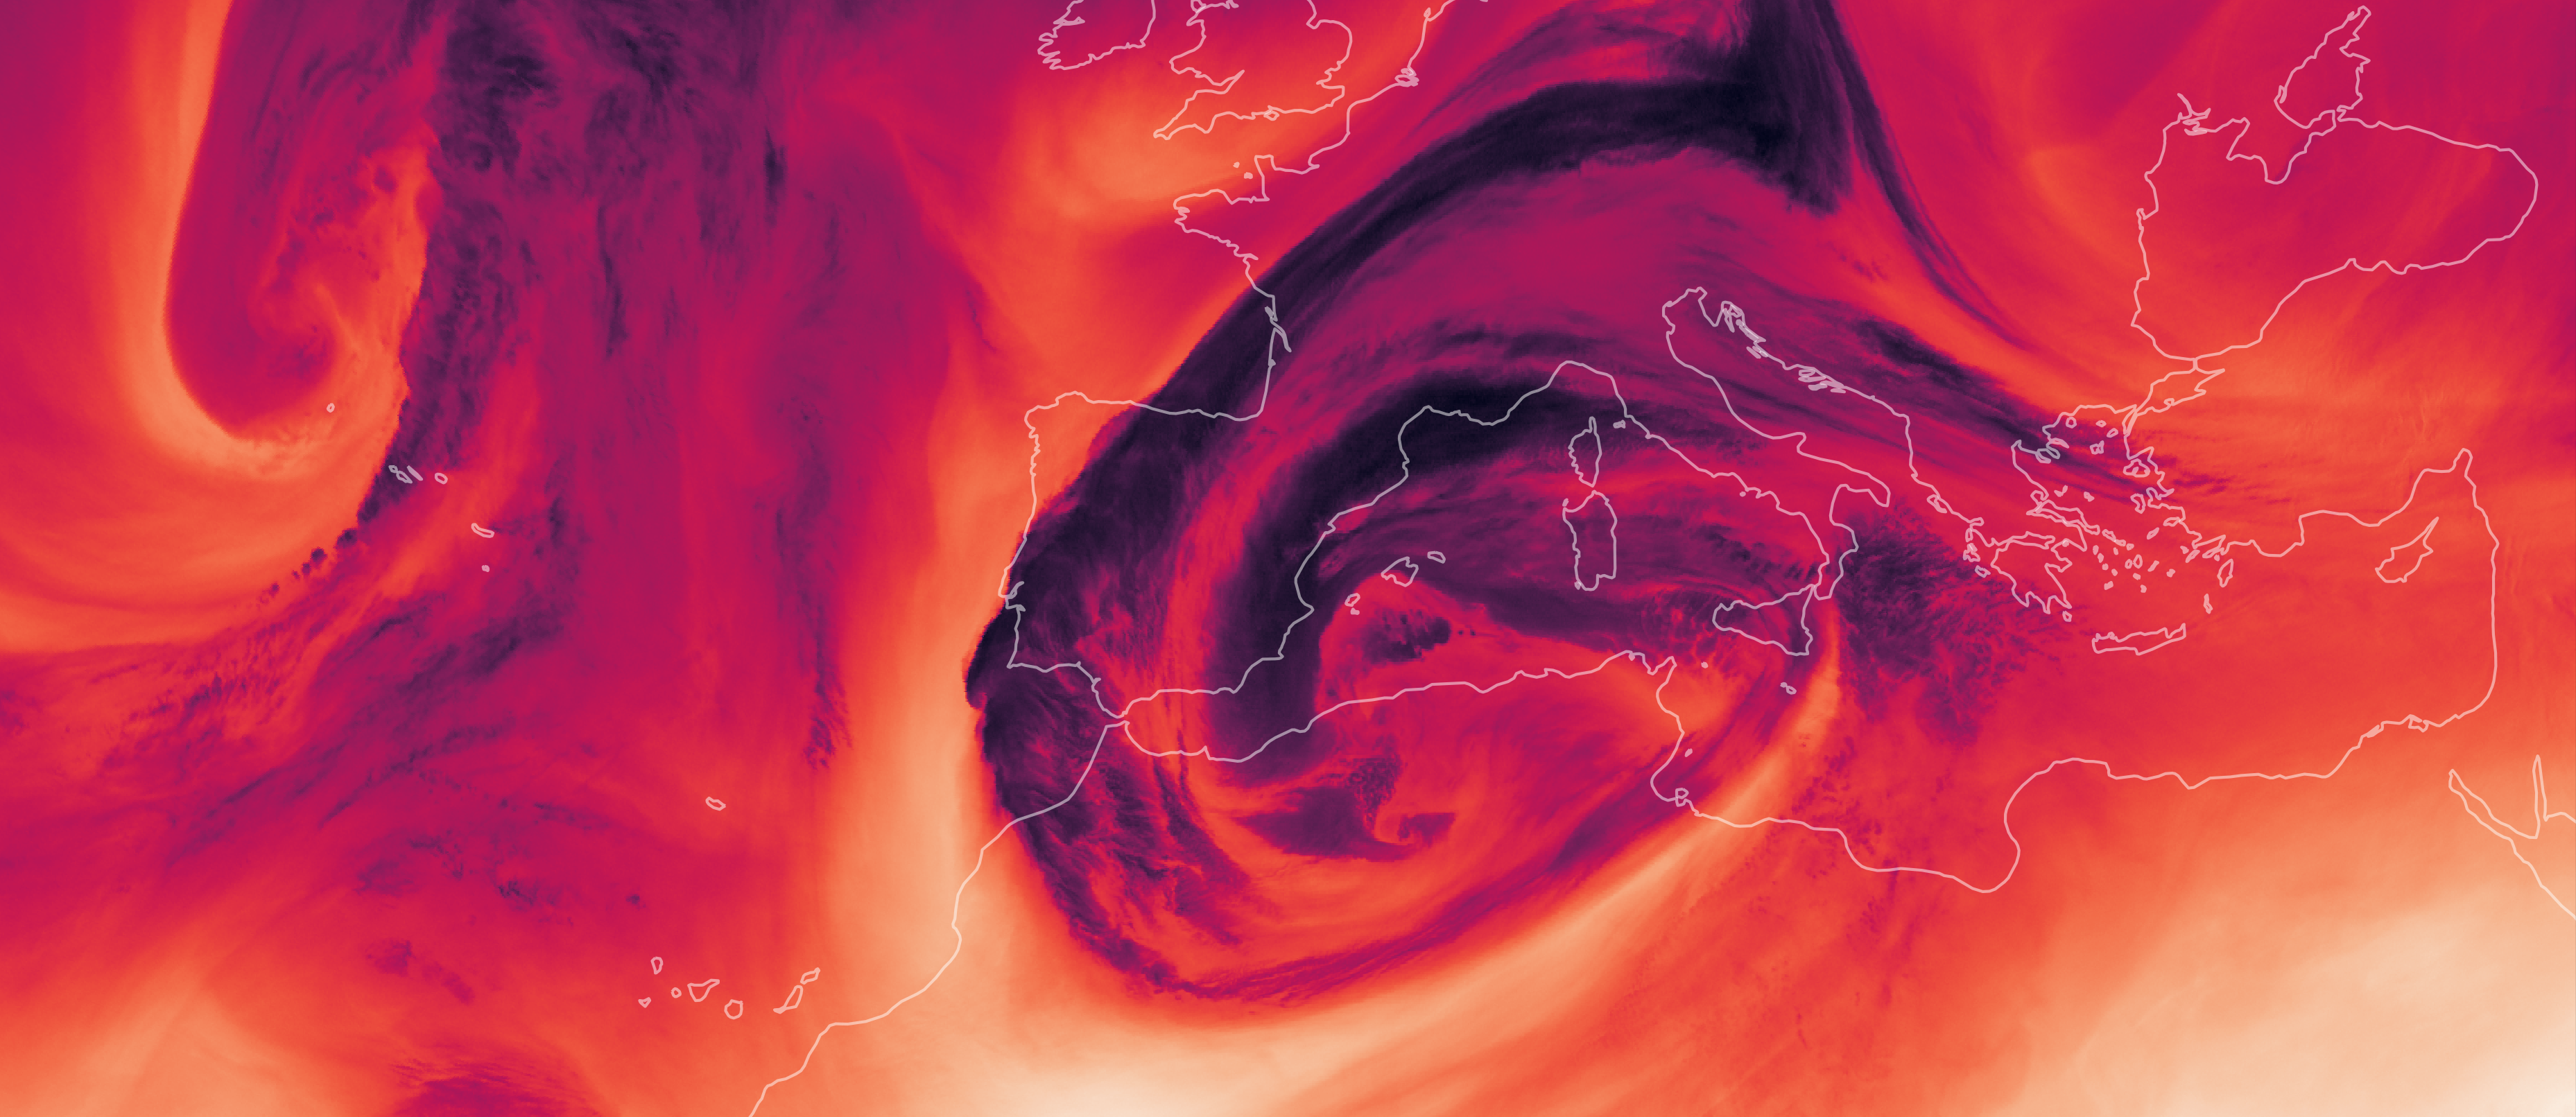
\includegraphics[width=\textwidth]{water_vapor}
\caption{Water vapor (white to red) and high clouds (purple to black) over the
Mediterranean as observed by the Spinning Enhanced Visible and Infrared
Imager at a wavelength of $\SI{6.2}{\micro \meter}$.}
\label{fig:introduction:water_vapor}
\end{figure}

This example illustrates that an understanding of the processes that generate
the infrared radiation observed by a satellite allows an observer to infer
moisture content as well as the presence of high clouds in the atmosphere.
Formulated more generally: If a component of the atmosphere interacts
sufficiently strongly with radiation, it generates an electromagnetic signal
that can be measured using a suitable sensor. By inverting the component's
interaction with the observed radiation, these measurements can be used to infer
the properties defining the interaction. This inversion process is
called \textit{the retrieval} and is required to relate satellite observations
to the physical state of the atmosphere.

The subject of this thesis are computational methods for the retrieval of
properties of clouds and precipitation from satellite observations. As will be
explained in more detail later on, these measurements are difficult, firstly,
due to the high variability in the appearance and composition of clouds and,
secondly, because of the complexity of their interaction with radiation. At the
same time, the important role that clouds and precipitation play in the weather
and climate system makes these measurements highly relevant for science and
society.

To set the scene for the discussion of satellite observations and retrieval
techniques in the subsequent chapters, this introduction aims to provide an
overview of the relevance of observing and measuring clouds and precipitation
from space. Beginning with the societal significance of water, the discussion
will move on to the scientific relevance of observing water as it moves through
the atmosphere.

\section{Water as resource}

Water is essential to life on Earth. It is the bloodstream of the biosphere
\citep{falkenmark04} and a fundamental resource to all forms of human
societies. The largest part of human freshwater consumption from lakes, rivers
or ground water, so called \textit{blue water} consumption, is used to irrigate
crops, while domestic and industrial use play minor roles. Blue water
consumption is distinguished from green water consumption, which refers to the
part of precipitation which is involved in the photosynthesis process. Although
rarely considered in consumption inventories, green water plays an important
role in providing water for rain-fed agriculture, which accounts for $60$ to
$\SI{70}{\percent}$ of the global food production, as well as the sustaining
of terrestrial ecosystems \citep{falkenmark04}.

Humans depend on water for food production both through irrigation from
blue water flows as well as the provision of soil moisture by green water flows.
Achieving food security has been recognized by the United Nations (UN) as a
sustainable development goal (SDG, \citeauthor{sdg}, \citeyear{sdg}). The large
contribution of food production to overall water consumption poses a challenge
to the management of water resources. Diverting more blue or green water flows
for the production of food reduces the amount of water that is available to
sustain terrestrial and aquatic ecosystems. There is thus direct potential for
conflict between SDG number two to end hunger and the SDGs 14 and 15 to sustain
terrestrial and aquatic ecosystems.

At the same time, water requirements for the production of energy are expected
to increase as fossil fuels are increasingly sourced from unconventional
deposits, such as shale oil and gas, whose extraction consumes substantial
amounts of water \citep{rosa18}. This is accompanied by a projected increase in
hydropower \citep{zarfl15} and the use of biofuels, both of which are reliant on
and affect freshwater supplies. This emerging competition in water uses is
recognized as the \textit{food-energy-water} nexus \citep{dodorico18}.


% Also here satellite observations that allow
%the monitoring of water resource are an important tool for the effective
%management of droughts \citep{boyd13}.

%Water consumption is typically categorized into two classes: blue and
%green water consumption. Blue water consumption refers to 
%
%The consumption of water is typically categorized as blue water consumption,
%which refers to the extraction of surface water from rivers or ground water, and
%green water consumption, which refe to rain water consumed directly, for example
%to grow crops. Of the global blue water consumption, agricultural activity
%constitutes the largest part followed by industrial activity and domestic use
%\citep{falkenmark04}. Agriculture, however, also consumes large amounts of
%green water as $60$ to $\SI{70}{\percent}$ of the world's  food is produced on
%rainfed land.
%
%Water also plays an important role as source of energy. In the year 2020, energy
%produced from hydroelectric plants constituted one sixth of the global energy
%production \citep{eia21} and it can be expected that this portion will increase
%with the required decarbonization of the energy sector.


\section{The hydrological cycle}

Sustainable human water consumption depends on the replenishment of the sources
from which water is obtained. Fresh water over land exists in the form of
glaciers, ice sheets, lakes and reservoirs, snow pack, wetlands and rivers as
well as a small part contained in the biomass. Water also exists within the land
surface in the form of soil moisture, permafrost and ground water. The largest
part of the water that is available on the surface of the Earth is stored in the
oceans. Only a very small part is stored in the atmosphere. Most that is in
the form of water vapor and only a minor fraction is contained in clouds in the
form of liquid droplets or ice crystals \citep{abbott19}.

Despite containing only a tiny fraction of the global water reserves at any
given moment, the atmosphere is responsible for essentially all of the water
transport from oceans to land, where it may precipitate to replenishes the water
storages from which it is available for direct or indirect consumption. The
system of fluxes between the different forms in which water exists on the
surface of the Earth is referred to as the hydrological cycle.

The illustration in Fig.~\ref{fig:introduction:water_cycle} provides an overview
of the atmospheric branch of the hydrological cycle, which is responsible for
the transport of water from the oceans to the land. The largest flux is the
influx of water vapor by evaporation from the ocean surface. Most of the water
vapor that evaporates over the ocean never reaches the land but instead returns
to it in form of precipitation. Only about $\SI{10}{\percent}$ of the
evaporation over oceans is transported to land, where it may form precipitation. A
significant part of that precipitation evaporates again allowing it to take part
in the formation of precipitation further inland.

\begin{figure}
\centering
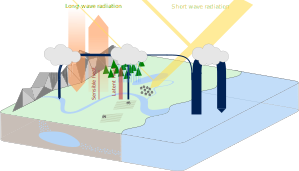
\includegraphics[width=0.8\textwidth]{water_cycle_energy}
\caption{
Illustration of the atmospheric branch of the hydrological cycle. Dark blue
arrows show the flow of water into, within and out of the atmosphere. Their
width approximately represents the strengths of these fluxes. The
semi-transparent arrows in orange, yellow and red show the energy fluxes in the
Earth system, which are directly coupled to the hydrological cycle by through
the radiative effects of water vapor, clouds and the release of latent heat.}
\label{fig:introduction:water_cycle}
\end{figure}

On the scale of river basins, the inflow of water through the atmosphere is the
only sustainable source of fresh water \citep{falkenmark04}. Given the competing
water requirements for the production of food and energy as well as ensuring
access to clean water and  sustaining of ecosystems, it is clear that water
management is required to avoid conflicts, minimize human suffering and reduce
ecological damage. This management has to rely on the monitoring and modeling of
the hydrological cycle. Since water fluxes within the hydrological cycle are
highly variable in space and time and occur across continental scales, satellite
observations are currently the only way through which continuous monitoring of
the hydrological cycle can be realized.


\section{Weather and climate}

Water in its various forms is a fundamental component of the Earth's weather
\citep{stevens13}.
When it evaporates, it takes up energy from the environment. This energy, the
latent heat, is released when the air cools and the water vapor condensates. The
release of latent heat acts as fuel for the development of vigorous convective
storms. The water that is released by those storms in the form of precipitation
can cause flooding and land slides.

The ability to predict the weather has considerable value for society,
especially for high impact events involving extreme wind speeds and
precipitation. The availability of satellite observations has played an
important role in the steady improvement of weather forecasts that occurred
during the last three decades
\citep{bauer15}. Weather forecasting  systems use satellite data to
determine a best estimate of the current state of the atmosphere, which is then
evolved into the future to predict the weather. While advanced forecasting
systems ingest satellite observations directly and are thus not dependent on
satellite retrievals \citep{bauer10}, some systems use retrieved cloud
properties for the initialization of short-range forecasts
\citep{dehaan14, benjamin21}. Besides that, retrievals of precipitation and
cloud properties are used by weather forecasters to gain situational awareness
and assess potential weather hazards.

%Despite the progress of the last decades, weather forecasts still struggle to
%produce accurate forecasts for specific meteorological contexts
%\citep{schafler18}. In many of those, the misrepresentation of the
%interaction of latent heat release through condensation and the large scale
%dynamics of the atmosphere were found \citep{rodwell13} to play a role.
%Improving the forecasts requires improving the representation of these processes
%in the model, which is where satellite-derived measurements of precipitation and
%clouds can help researchers better understand them.

At the same time, water also has a pivotal role in the climate system. As
illustrated in Fig.~\ref{fig:introduction:water_cycle}, it is coupled to the
Earth's energy budget by multiple effects. Water vapor is the most potent
greenhouse gas and thus contributes strongly to the retention of radiative
energy emitted from the Earth's surface. In the form of clouds, water both cools
the Earth system through the reflection of solar radiation and warms it through
the absorption of upwelling longwave radiation. Although the global effect of
clouds is a pronounced cooling, the effect varies regionally and with the
properties of the clouds. Evaporation, transpiration and convection are
important for the transfer of heat from the Earth's surface to the atmosphere.
Since, on average, evaporation and transpiration have to be balanced by
precipitation, the energy budget of the Earth is directly linked to
precipitation \citep{trenberth09}.

Instead of a passive tracer of atmospheric dynamics, water must thus be
understood an active component of the both the weather and the climate system
and thus links these systems to the hydrological cycle. Because of the global
extent and complex nature of these systems, satellite observations of the
hydrological cycle are essential for climate science and meteorology.

\section{A warmer planet}

As a consequence of anthropogenic emissions of carbon dioxide, the Earth's
 climate is warming. As the Earth system adapts to the increased radiative
 forcing from greenhouse gases, its climate changes. These changes are not
 uniform but exhibit strong regional variability. Reliable regional predictions
 of climate change are required to help societies adapt to the changing climate.
 However, the current understanding as well as the ability to predict changes at
 regional scales remains severely limited.

The hydrological cycle will change together with the climate. Because of the
ability of warmer air to hold more water, water vapor concentrations are
increasing. An increase in evaporative demand is expected lead to more frequent
and severe droughts. At the same time global precipitation is expected to
increase. Extreme precipitation events are strengthening and becoming more
frequent. At the scales of individual precipitation systems, precipitation
increases with the capacity of warmer air to carry water vapor. Globally,
however, evapotranspiration and thus also precipitation are constrained by the
Earth's energy budget, which limits increases in global precipitation to a lower
rate than that of individual storms \citep{collins13}. In addition to that,
changes in the general circulation will modify the global distribution of
precipitation.

As part of the hydrological cycle, clouds will change with the climate. Since
clouds reflect incoming solar radiation and the absorb outgoing long-wave
radiation, these changes act as a feed back on the Earth's energy budget and
will thus influence the response of the climate system to increased CO$_2$
concentrations. Whether an individual cloud exerts a net warming or cooling
effect on the climate system depends on its properties such as altitude and
composition as well as its location. The representation of clouds remains an
important challenge for climate models and uncertainties in cloud feedbacks
remain the primary source of uncertainty in predictions of the climate response
to increased CO$_2$ concentrations in the atmosphere \citep{zelinka20}.

The understanding of climate change has progressed immensely during the last
decade but remains insufficient to make confident predictions at regional
scales. Such predictions are necessary for successful climate change adaptation.
Satellite observations are essential for improving and validating climate models
and the monitoring of changes in the climate system. This makes them a crucial
guide for the passage into an uncertain, warmer future.

\section{Why satellites?}

Considering the importance of rain for a large range of human activities, it is
not surprising that humans have been measuring precipitation and trying to
improve their understanding of the weather system. The most direct and arguably
intuitive way to measure precipitation is through the use of \textit{rain
gauges}. A rain gauge consists of a cavity, which captures rain and from which
the accumulated precipitation can be measured. First records of gauge
measurements of rain date back to as long as 400 years
BC \citep{strangeways2000}. Today, gauge measurements are available from all
continents, however their density varies from country to country and is
oftentimes tied to the local population density.

The main disadvantage of rain gauges is the highly localized character of their
measurements, which limits their ability to accurately capture the spatial
structure of precipitation on short time scales. Moreover, because these
measurements are performed by a large number of public and entities actors across
the globe, not all of them are easily accessible for scientists. Effectively,
only $\SI{1}{\percent}$ of the surface of the Earth is estimated to be within a
distance of $\SI{5}{\kilo \meter}$ from the nearest gauge
measurement \citep{kidd17}.

Over land, another important technique for measuring precipitation are
ground-based radars. These radars send out beams of radiation, which are
reflected by rain and snow. Precipitation within a radius several hundreds of
kilometers from the radar can be detected by measuring the amount of radiation
that is reflected back to the radar. Over land, ground-based radars are
important for the real-time monitoring of precipitation. However, due to their
high installation and maintenance costs, their spatial availability is irregular
and typically follows the local population density. In addition to that, the
availability and accuracy of radar measurements may be hampered by complex
terrain as well as the distance from the radar location, which limits the
usefulness of these observations for climatological applications.

The relevance of clouds and precipitation for the hydrological cycle has been
known since before the times of Aristotle \citep{frisinger72}. Nonetheless, the
systematic study of clouds has long remained a secondary focus of
meteorology and it took until the 1970s before the importance of interactions
between clouds, weather and climate put them at the forefront of atmospheric and
climate research \citep{stephens03}. Traditionally, cloud observations were
conducted as parts of routine meteorological observations performed on land and
ships \citep{hughes84}. However, these observations were mostly qualitative in
nature indicating only the presence of clouds, their type and an  approximate
height.

The principal drawback of the measurement techniques discussed above is their
limited and irregular spatial coverage. This reduces their suitability for the
monitoring of global weather and climate. Satellites have the ability to provide
observations across the globe at high temporal resolutions. Because of this they
ideally complement ground-based measurements and have become an essential source
of information for a wide range of scientific, economic and societal activities.

